\chapter{Exhaustive search of binary sequences}
  \section{Previous work}

  As shown in the previous chapter, algebraic constructions for sequences
  with  low off-peak autocorrelation have huge constraints on the length of
  the generated sequences. To overcome this limitation, exhaustive searches
  through all possible candidates for a given length have been conducted in the past. The size of the search space in this case is  $O(2^n)$, where $n$ is the length of the binary sequence, which make their
 results very costly in terms of computational complexity.\\

For a similar case there has been studies for finding sequences with low aperiodic autocorrelation, whereas fewer works has been done in the periodic autocorrelation due to the existance of the optimal algebraic constructions, which have been sufficient for past practical purposes. In the next paragraphs  we review the literature on the aperiodic autocorrelation.\\

 First of all, aperiodic autocorrelation  and the energy of a sequence  are defined as follows.\\
  \begin{definition}[Aperiodic autocorrelation]
      Given a binary sequence $S$, its aperiodic autocorrelation is defined as:
      \begin{equation}
        A'_{\tau}(S) = \sum_{i=0}^{n-\tau-1}s_{i}s_{i+\tau}
      \end{equation}
  \end{definition}

  \begin{definition} Given a binary sequence $S$, the energy of $S$ is defined
    as:
    \begin{equation}
      E(S) = \sum_{k=1}^{n-1} A'_{k}(S)^{2}
    \end{equation}

  \end{definition}
The idea is finding the sequence $S$ belonging to a given set of possible sequences that gives the minimum posible energy through the branch and bound with objetive function
     \begin{equation}
      E_{min} = \operatorname*{min}_{subset} \sum_{k=1}^{n-1} A'^{2}_{k}.
    \end{equation}

An improvement for this method was   proposed by \citet{Mertens_1996} in which he provided an algorithm  with complexity  $O(1.85^n)$. In his work, he applied a branch and bound
approach that rules out equivalent sequences and uses an heuristic based on how complementing a single symbol of the sequence affects the autocorrelation.\\

  First of all, the recursion is done by choosing a sequence and recursively
  fixing the elements at both ends  of the sequence as shown in Figure
  \ref{prn_search:fig:1}.\\

  \begin{figure}[ht!]
    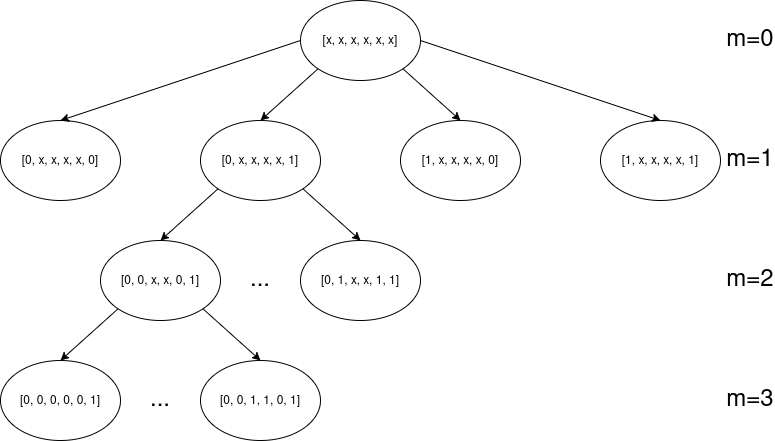
\includegraphics[scale=0.6]{Chapters/prn_search/branching_example.png}
    \caption{An example of the branching used in \citet{Mertens_1996} with
    $n = 6$ and where x represent unfixed values.}
    \label{prn_search:fig:1}
  \end{figure}

  When a symbol of the original sequence is complemented,
  the components of the autocorrelation can be decremented by, at most, 2. Based on
  that, a relaxation of $E_{min}$ can be proposed:\\
  \begin{equation}
    E_b = \sum_{k=1}^{n-1}max\{b_k, (|A'_k| - 2f_k)^2\} \leq E_{min}
  \end{equation}
  where $A'_k$ is the autocorrelation of an arbitrary sequence, $b_k = (n -
  k) \bmod 2$ the minimum possible value for $|A'_k|$ and $f_k$ the number of
  unfixed elements in $A'_k$ given by:
  \begin{equation}
    f_k = \left\{\begin{array}{ll}
        0 & k \geq N - m \\
        2(n - m - k) & n/2 \leq k < n - m\\
        n - 2m & k < n/2 \\
    \end{array}\right.
  \end{equation}

  where $n$ is the size of the sequence to search and $m$ the number of fixed
  elements at the ends of the sequence.\\

  If $E_b$ is greater than the best candidate for $E_{min}$ so far, that branch
  can be pruned reducing the amount of computation. With this algorithm,
  Mertens succesfully computed sequences up to length $n = 48$.\\

  This work was further improved by \citet{Packebusch_2016} combining bounds provided by different authors (Prestwich and
  Wiggenbrock) to create a new bound and  lowering the
  complexity to $O(1.729^n)$ obtaining sequences of length  $n= 66$. This
  record was broken by \citet{anatoli} by computing sequences up to length $n = 85$.\\

  \section{Our approach}

  To tackle the huge complexity encountered in the previous methods, a different
  approach was taken. Instead of dealing with the combinatorial explosion
  of all the possible binary sequences of length $n$, we decided to work with
  a smaller set consisting on all the possible sequences which can be
  constructed through the composition method with Legendre base sequences.\\

  This approach haves some pros and cons. First of all, the search space is
  reduced from $O(2^n)$ to $O(p^m)$ where $p \cdot m = n$. This clearly means that
  the complexity grows slower than in previous works. In fact, the
  autocorrelation function can be optimized for sequences generated through the
  composition method as shown in Chapter \ref{chap:computational_analysis}.\\

  The problem is that the possible lengths for the sequences are limited as $m$
  and $p$ are required to be coprime. Even though it means that
  these method cannot find optimal sequences for all lengths, the restriction is
  looser than the non-exhaustive methods. Apart from that, this method does not
  explore all possible permutations and it does not ensure to find a pseudonoise
  sequence if it exists. To sum up, this method is a good way to construct useful
  sequences but should not be used to prove the non existence of pseudonoise
  sequences for a given length.\\

  Given a base sequence of length $p$ and  shift sequences of length $m$ ,
  our program needs to find all the shift sequences that generate a composite
  sequence with a good autocorrelation.\\

  This means that the search space are all the posible permutations of the
  shift sequence, in other words, $p^m$ permutations. However, there are some
  relations between the different shift sequences that let us narrow the
  search space.\\

  For example, if a constant is added to every component of the shift sequence,
  a shifted version of the same sequence is obtained. This means that if only
   permutations that start with the same component are computed,
  then the whole search space would be covered as any other permutations would just
  be shifts of one permutation from the computed set. This optimization narrows
  our search space to $p^{(m-1)}$.\\

  Other optimization arises from the form of the shift sequences. In general,
  if the symbols are repeated often, they tend to generate higher
  autocorrelation spikes or periods inside the composite sequence. This
  concept can be easily expressed with the Hamming autocorrelation function:\\

  \begin{definition}[Hamming autocorrelation]
    Given a sequence $S$ of length $n$ and the  $shift$ function  defined at
    Equation \eqref{eq:3}, the Hamming autocorrelation is defined as:
      \begin{equation} \label{hamming:eq:1}
        HA(S)_{\tau} = \sum_{\tau = 0}^{n-1} HAComponent(S_{\tau}, shift(S, \tau)_{\tau})
      \end{equation}
    where $HAComponent$ is defined as:
      \begin{equation}
        HAComponent(c1, c2) = \left\{\begin{array}{lr}
            1  &  c1 = c2\\
            0  & \textnormal{otherwise} \\
        \end{array}\right.
      \end{equation}
  \end{definition}

  For our branch and bound algorithm, it is important to note that if a symbol
  that only appears once is substituted for another, the hamming
  autocorrelation won't get lower. This means that if a depth-in-first
  bounding of the nodes that have a hamming autocorrelation higher than the
  threshold (we mean, the maximum non trivial component) is performed,
  all nodes in that branch are ensured to have a higher hamming autocorrelation
  than the threshold.\\

  \begin{figure}[ht!]
    \begin{center}
      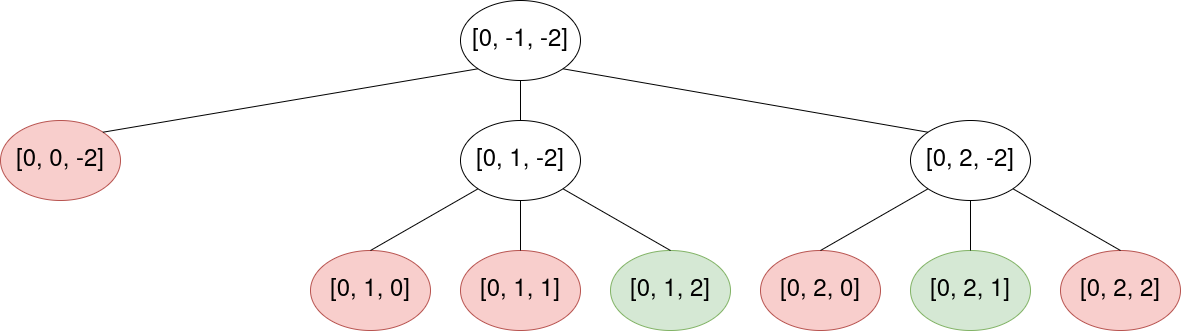
\includegraphics[scale=0.4]{Chapters/Implementation/Example_branch_bound.png}
    \end{center}
    \caption{An example of the branch and bound algorithm with a threshold for
    hamming autocorrelation of 1 and a base sequence of length 3. Red nodes
    represent prunes and green ones final nodes in which the
    autocorrelation is computed and checked. Negative values represent those
    that haven't been initialized yet.}
    \label{bb:fig:1}
  \end{figure}

  Some properties of the algorithm can be deduced from Figure \ref{bb:fig:1}.
  First of all, the number of autocorrelations computed can be reduced by a
  significant amount. However, the computation on each branch isn't balanced. This
  must be taken into account when the parallelism model is designed.
